\chapter{Bmad Concepts and Organization}
\label{c:lat.concepts}

This chapter is an overview of some of the nomenclature used by \bmad. Presented are the basic
concepts, such as \vn{element}, \vn{branch}, and \vn{lattice}, that \bmad uses to describe such
things as LINACs, storage rings, X-ray beam lines, etc.

%---------------------------------------------------------------------------
\section{Lattice Elements}
\label{s:element.def}

\index{lattice element}
\index{element}
\index{controller element}
The basic building block \bmad uses to describe a machine is the \vn{lattice} \vn{element}. An
element can be a physical thing that particles travel ``through'' like a bending magnet, a
quadrupole or a Bragg crystal, or something like a \vn{marker} element (\sref{s:mark}) that is used
to mark a particular point in the machine.  Besides physical elements, there are \vn{controller}
elements (Table~\ref{t:control.classes}) that can be used for parameter control of other elements.

Chapter~\sref{c:elements} lists the complete set of different element types that \bmad knows about.

\index{beginning element}\index{end element}
In a lattice \vn{branch} (\sref{s:branch.def}), The ordered array of elements are assigned a number
(the element index) starting from zero. The zeroth \vn{beginning_ele} (\sref{s:begin.ele}) element,
which is always named \vn{BEGINNING}, is automatically included in every branch and is used as a
marker for the beginning of the branch.  Additionally, every branch will, by default, have a final
marker element (\sref{s:mark}) named \vn{END}.

%---------------------------------------------------------------------------
\section{Lattice Branches}
\label{s:branch.def}

\index{branch}
The next level up from a \vn{lattice} \vn{element} is the \vn{lattice} \vn{branch}. A \vn{lattice}
\vn{branch} contains an ordered sequence of lattice elements that a particle will travel through. A
branch can represent a LINAC, X-Ray beam line, storage ring or anything else that can be represented
as a simple ordered list of elements.

Chapter~\sref{c:sequence} shows how a \vn{branch} is defined in a lattice file with \vn{line},
\vn{list}, and \vn{use} statements.

A \vn{lattice} (\sref{s:lattice.def}), has an array of \vn{branches}. Each \vn{branch} in this array
is assigned an index starting from 0. Additionally, each \vn{branch} is assigned a name which is the
\vn{line} that defines the branch (\sref{s:use}).

%---------------------------------------------------------------------------
\section{Lattice}
\label{s:lattice.def}

\index{lattice}\index{branch} 
an array of \vn{branches} that can be interconnected together to describe an entire machine
complex. A \vn{lattice} can include such things as transfer lines, dump lines, x-ray beam lines,
colliding beam storage rings, etc. All of which are connected together to form a coherent whole. In
addition, a lattice may contain \vn{controller elements} (Table~\ref{t:control.classes}) which can
simulate such things as magnet power supplies and lattice element mechanical support structures.

\index{root branch}
Branches can be interconnected using \vn{fork} and \vn{photon_fork} elements (\sref{s:fork}). This
is used to simulate forking beam lines such as a connections to a transfer line, dump line, or an
X-ray beam line. The \vn{branch} from which other \vn{branches} fork is called a \vn{root} branch.

A lattice may contain multiple \vn{root} \vn{branches}. For example, a pair of intersecting storage
rings will generally have two \vn{root} branches, one for each ring. The \vn{use} statement
(\sref{s:use}) in a lattice file will list the \vn{root} \vn{branches} of a lattice. To connect
together lattice elements that are physically shared between branches, for example, the interaction
region in colliding beam machines, \vn{multipass} lines (\sref{s:multipass}) can be used.

The root branches of a lattice are defined by the \vn{use} (\sref{s:use}) statement. To further
define such things as dump lines, x-ray beam lines, transfer lines, etc., that branch off from a
root branch, a forking element is used.  \vn{Fork} elements can define where the particle beam can
branch off, say to a beam dump. \vn{photon_fork} elements can define the source point for X-ray
beams.  Example:
\begin{example}
  erl: line = (..., dump, ...)               ! Define the root branch 
  use, erl
  dump: fork, to = d_line                    ! Define the fork point
  d_line: line = (..., q3d, ...)             ! Define the branch line
\end{example}

Like the root branch \bmad always automatically creates an element with \vn{element index} 0 at the
beginning of each branch called \vn{beginning}. The longitudinal \vn{s} position of an element in a
branch is determined by the distance from the beginning of the branch.

Branches are named after the line that defines the \vn{branch}. In the above example, the branch
line would be named \vn{d_line}. The root branch, by default, is called after the name in the
\vn{use} statement (\sref{s:use}).

The ``branch qualified'' name of an element is of the form
\begin{example}
  branch_name>>element_name
\end{example}
where \vn{branch_name} is the name of the branch and \vn{element_name} is the ``regular'' name of
the element. Example:
\begin{example}
  root>>q10w
  xline>>cryst3
\end{example}
When parsing a lattice file, branches are not formed until the lattice is expanded
(\sref{s:expand}). Therefore, an \vn{expand_lattice} statement is required before branch qualified
names can be used in statements. See \sref{s:ele.match} for more details.

%---------------------------------------------------------------------------
\section{Lord and Slave Elements}
\label{s:lord.slave}

\begin{figure}[tb]
 \begin{center}
 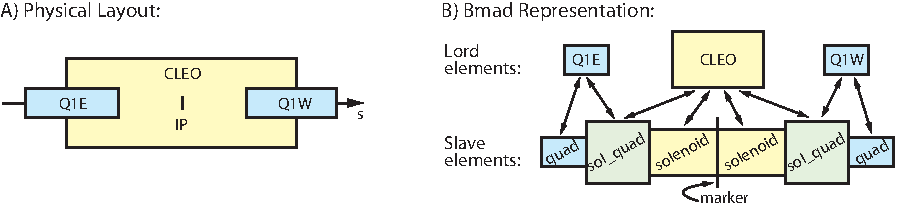
\includegraphics[width=6.0in]{superimpose-ip.pdf}
 \caption[Superposition example.]{
Superposition Example. A) Interaction region layout with quadrupoles overlapping a solenoid. B) The
Bmad lattice representation has a list of split elements to track through and the undivided ``lord''
elements. Pointers (double headed arrows), keep track of the correspondence between the lords and
their slaves.
 }
 \label{f:super.ip}
 \end{center}
 \end{figure}

%---------------------------------------------------------------------------

A real machine is more than a collection of independent lattice elements. For example, the field
strength in a string of elements may be tied together via a common power supply, or the fields of
different elements may overlap.

\bmad tries to capture these interdependencies using what are referred to as \vn{lord} and
\vn{slave} elements. The \vn{lord} elements may be divided into two classes. In one class are the
\vn{controller} elements.  These are \vn{overlay} (\sref{s:overlay}), \vn{group} (\sref{s:group}),
\vn{ramper} (\sref{s:ramper}), and \vn{girder} (\sref{s:girder}) elements that control the
attributes of other elements which are their slaves.

The other class of \vn{lord} elements embody the separation of the physical element from the track
that a particle takes when it passes through the element. There are two types

An example will make this clear.  \vn{Superposition} (\sref{s:super}) is the ability to overlap
lattice elements spatially. \fig{f:super.ip} shows an example which is a greatly simplified version
of the IR region of Cornell's CESR storage ring when CESR was an e+/e-- collider. As shown in
\fig{f:super.ip}A, two quadrupoles named \vn{q1w} and \vn{q1e} are partially inside and partially
outside the interaction region solenoid named \vn{cleo}. In the lattice file, the IR region layout
is defined to be
 {\small
\begin{example}
  cesr: line = (... q1e, dft1, ip, dft1, q1w ...)
  cleo: solenoid, l = 3.51, superimpose, ref = ip
\end{example}
 }
The line named \vn{cesr} ignores the solenoid and just contains the interaction point marker element
named \vn{ip} which is surrounded by two drifts named \vn{dft1} which are, in turn, surrounded by
the \vn{q1w} and \vn{q1e} quadrupoles. The solenoid is added to the layout on the second line by
using superposition. The ``ref = ip'' indicates that the solenoid is placed relative to \vn{ip}. The
default, which is used here, is to place the center of the superimposed \vn{cleo} element at the
center of the \vn{ip} reference element.  The representation of the lattice in \bmad will contain
two branch \vn{sections} (``sections'' is explained more fully later): One section, called the
\vn{tracking section}, contains the elements that are needed for tracking particles. In the current
example, as shown in \fig{f:super.ip}B, the first IR element in the tracking section is a quadrupole
that represents the part of \vn{q1e} outside of the solenoid. The next element is a combination
solenoid/quadrupole, called a \vn{sol_quad}, that represents the part of \vn{q1e} inside \vn{cleo},
etc.  The other branch section that Bmad creates is called the \vn{lord section} This section
contain the undivided ``physical'' \vn{super_lord} elements (\sref{s:super}) which, in this case are
\vn{q1e}, \vn{q1w}, and \vn{cleo}. Pointers are created between the lords and their \vn{super_slave}
elements in the tracking section so that changes in parameters of the lord elements can be
transferred to their corresponding slaves.

\vn{super_lord}s are used when there are overlapping fields between elements, the other case where
there is a separation between the physical (lord) element and the (slave) element(s) used to track
particles through comes when a particle passes through the same physical element multiple times such
as in an Energy Recovery Linac or where different beams pass through the same element such as in an
interaction region. In this case, \vn{multipass_lords} representing the physical elements and
\vn{multipass_slaves} elements which are used for tracking can be defined (\sref{s:multipass}).
Superposition and multipass can be combined in situations where there are overlapping fields in
elements where the particle passes through

\index{no_major_lord}\index{multipass_slave}\index{slice_slave}\index{super_slave}
\index{not_a_lord}\index{group_lord}\index{girder_lord}\index{overlay_lord}
\index{multipass_lord}\index{super_lord}\index{slave_status}\index{lord_status}
Each lattice element is assigned a \vn{slave_status} indicating what kind of slave it is and a
\vn{lord_status} indicating what kind of lord it is. Normally a user does not have to worry about
this since these status attributes are handled automatically by \bmad.  The possible
\vn{lord_status} settings are:
  \begin{description}
  \item[girder_lord]\Newline 
A \vn{girder_lord} element is a \vn{girder} element  (\sref{s:girder}). 
  \item[multipass_lord]\Newline
\vn{multipass_lord} elements are created when
multipass lines are present (\sref{s:multipass}). 
  \item[overlay_lord]\Newline 
An \vn{overlay_lord} is an \vn{overlay} element (\sref{s:overlay}). 
  \item[group_lord]\Newline 
A \vn{group_lord} is a \vn{group} element (\sref{s:group}).
  \item[super_lord]\Newline 
A \vn{super_lord} element is created when elements are
superimposed on top of other elements (\sref{s:super}).
  \item[not_a_lord]\Newline
This element does not control anything.
  \end{description}
Any element whose \vn{lord_status} is something other than
\vn{not_a_lord} is called a \vn{lord} element. In the \vn{tracking part}
of the branch, \vn{lord_status} will always be
\vn{not_a_lord}. In the \vn{lord section} of the branch, under normal
circumstances, there will never be any \vn{not_a_lord} elements.

Lord elements are divided into two classes.  A \vn{major} lord represents a physical element which
the slave elements are a part of.  \vn{super_lord}s and \vn{multipass_lord}s are \vn{major} lords.
As a consequence, a \vn{major} lord is a lord that controls nearly all of the attributes of its
slaves.  The other lords --- \vn{girder_lord}s, \vn{group_lord}s and \vn{overlay_lord}s --- are
called \vn{minor} lords.  These lords only control some subset of a slaves attributes.

The possible \vn{slave_status} settings are
  \begin{description}
  \item[multipass_slave]\Newline
A \vn{multipass_slave} element is the slave of a \vn{multipass_lord}
(\sref{s:multipass}).
  \item[slice_slave]\Newline
A \vn{slice_slave} element represents a longitudinal slice of another element.
Slice elements are not part of the lattice but rather are created on-the-fly
when, for example, a program needs to track part way through an element.
  \item[super_slave]\Newline 
A \vn{super_slave} element is an element in the tracking part of the branch that 
has one or more \vn{super_lord} lords (\sref{s:super}).
  \item[minor_slave]\Newline
\vn{minor_slave} elements are elements that are not \vn{slice_slave}s and are only controlled
by \vn{minor} lords (\vn{overlay_lord}s, \vn{group_lord}s, or \vn{girder_lord}s).
  \item[free]\Newline
A \vn{free} element is an element with no lords.
  \end{description}

For historical reasons, each \vn{branch} in a lattice has a \vn{tracking section} and a \vn{lord
section} and the \vn{tracking section} is always the first (lower) part of the element array and the
\vn{lord section} inhabits the second (upper) part of the array.  All the \vn{lord} elements are put
in the \vn{lord section} of branch 0 and all the other \vn{lord sections} of all the other branches
are empty.

As a side note, \'Etienne Forest's PTC code (\sref{s:ptc.intro}) uses separate structures to
separate the physical element, which PTC calls an \vn{element} from the particle track which PTC
call a \vn{fibre}.  [Actually, PTC has two structures for the physical element, \vn{element} and
\vn{elementp}. The latter being the ``polymorph'' version.] This \vn{element} and \vn{fibre}
combination corresponds to \bmad \vn{multipass_lord} and \vn{multipass_slave} elements. PTC does not
handle overlapping fields as \bmad does with \vn{superposition} (\sref{s:super}).

%---------------------------------------------------------------------------
\section{PTC: Polymorphic Tracking Code}
\label{s:ptc.intro}
\index{PTC}

The PTC/FPP library of \'Etienne Forest handles Taylor maps to any arbitrary order. This is also
known as Truncated Power Series Algebra (TPSA). The core Differential Algebra (DA) package used by
PTC/FPP was developed by Martin Berz\cite{b:berz}. The PTC/FPP libraries are interfaced to \bmad so
that calculations that involve both \bmad and PTC/FPP can be done in a fairly seamless manner.

Basically, the FPP (``Fully Polymorphic Package'') part of the code handles Taylor map
manipulation. This is purely mathematical. FPP has no knowledge of accelerators, magnetic fields,
particle tracking etc. PTC (``Polymorphic Tracking Code'') implements the physics and uses FPP to
handle the Taylor map manipulation. Since the distinction between \vn{FPP} and \vn{PTC} is
irrelevant to the non-programmer, ``PTC'' will be used to refer to the entire package.

PTC is used by \bmad when constructing Taylor maps and when the \vn{tracking_method}
\sref{s:tkm}) is set to \vn{symp_lie_ptc}. All Taylor maps above first order are calculated
via PTC. No exceptions.

For more discussion of PTC see Chapter~\sref{c:ptc.use}.  For the programmer, also see
Chapter~\sref{c:ptc.program}.

For the purposes of this manual, PTC and FPP are generally considered one package and
the combined PTC/FPP library will be referred to as simply ``PTC''.

%---------------------------------------------------------------------------
\section{Tao: Tool for Accelerator Optics Program}
\label{s:tao.intro}
\index{Tao}

The strength of \bmad is that, as a subroutine library, it provides a flexible framework from which
sophisticated simulation programs may easily be developed.  The weakness of \bmad comes from its
strength: \bmad cannot be used straight out of the box. Someone must put the pieces together into a
program. To partially remedy this problem, the \tao program\cite{b:tao} has been developed at
Cornell. \tao, which uses \bmad as its simulation engine, is a general purpose program for
simulating particle beams in accelerators and storage rings.  Thus \bmad combined with \tao
represents the best of both worlds: The flexibility of a software library with the ease of use of a
program.

